%%
%% @filename TD3.tex
%% @date jeu. 19 nov. 2020 14:58:12 CET
%% @author Guillaume Fornes <guillaume.fornes@enseirb-matmeca.fr>
%%
\documentclass[a4paper]{article}

\usepackage[utf8]{inputenc}
\usepackage[french]{babel} 

% Figures
\usepackage{graphicx}
\graphicspath{{./img/}}

% Math
\usepackage{amsmath, amssymb}
\newcommand\p{\bullet}
\usepackage{bussproofs}

% Algortihmes
\usepackage[vlined,lined,linesnumbered,boxed,french]{algorithm2e}
\DeclareMathOperator*{\argmin}{argmin}
\DeclareMathOperator{\myfunc}{myfunc}
\DeclareMathOperator*{\sign}{sign}
\DeclareMathOperator*{\imwh}{width}
\DeclareMathOperator*{\imht}{height}

% Extra
\usepackage[left=2cm,right=2cm,top=2cm,bottom=2cm]{geometry}
\usepackage{url}

\begin{document}
\part*{TD3 - Preuve formelle}
\vspace{1cm}
\section{Un calcul simple}
\vspace{5mm}
\subsection*{Exercice 1}
\begin{enumerate}
  \item $\dfrac{\dfrac{}{\p\p NDP \p}(Ax)}{\p\p NDP\p\p\p}(R_{1})$\\
  \item  $\dfrac{\p\p NDP \p\p}{\p\p NDP\p\p\p}(R_{1})$\\
  \item (Ax) : $n(xy) = n(x) + n(y) > n(x)$ \\
    donc $n(xy)$ ne divise pas $n(x)$\\

    $(R_1)$ Supposons que xNDPy prouvable et valide \\
    Par $(R_{1})$ xNDPxy est prouvable, montrons la validité \\
    Par l'absurde : supposons que $n(x)$ divise $n(xy)$\\
    $\implies n(xy)\: = k.n(x) \: \text{ pour un certain }k>1$\\
    $\iff n(x) + n(y) = k.n(x)$\\
    $\iff n(y) = (k-1).n(x)$\\
    Voir vidéo du chapitre \\
\end{enumerate}
\subsection*{Exercice 2}
\begin{enumerate}
  \item {\large$\dfrac{\dfrac{\dfrac{}{\p\p\p NDP \p\p}(Ax)}{\p\p\p NDP\p\p\p\p\p}(R_{1})\text{      } \dfrac{\dfrac{\dfrac{\dfrac{}{\p\p NDP \p}(Ax)}{\p\p NDP \p\p\p}(R_{1})}{\p\p  NDP\p\p\p\p\p}(R_{1})}{\p\p\p\p\p SD\p\p}(R_{3})}{\p\p\p\p\p SD\p\p\p}(R_{3})$}\\
  \item (vidéo du cours)\\
\end{enumerate}
\subsection*{Exercice 3}
\begin{enumerate}
  \item $\dfrac{\dfrac{\dfrac{\dfrac{}{\p\p\p NDP \p}(Ax)}{\p\p NDP \p\p\p}(R_{1})}{\p\p\p SD \p\p}(R_{2})}{P\p\p\p}(R_{4})$\\
  \item (vidéo du cours)\\
\end{enumerate}\newpage
\section{Calcul des séquents propositionnels}
\vspace{5mm}
\subsection*{Exercice 4}
\begin{enumerate}
  \item $\dfrac{\dfrac{}{A, B \vdash A}(R1) \dfrac{}{A,B \vdash B}(R1)}{A,B\vdash (A\land B)}(R7.1)$\\
    Soit v une valuation de A et B. \\Si v(A)=1 et v(B)=1 \\
    alors $[A\land B]_v=[A]_v.[B]_v=v(A).v(B)=1$\\
  \item $\dfrac{\dfrac{}{A,(A\implies B)\vdash A \implies B}(R1) \; \dfrac{}{A, (A\implies B) \vdash A}(R1)}{A,(A\implies B) \vdash B}(R3)$\\
  \item $\dfrac{}{A,B,(A\implies B \implies C) \vdash C}(R)$ (Comme le précedent mais avec une étape de plus.)\\
    Faisons donc une preuve sémantique de cette question.\\
    On prends v une valuation quelconque.
    Si $A,B$ et $A\implies( B\implies C)$ sont vraies dans v,\\
    alors $B\implies C$ vraie dans v,
    alors $C$ est vraie dans V.\\
  \item $\dfrac{\dfrac{\dfrac{}{A,A\implies C, B\implies C \vdash C}(R1) \dfrac{}{A,A\implies C, B \implies C \vdash A}(R1)}{A,(A\implies C), (B\implies C)\vdash C}(R3)\dfrac{\text{symétrique à l'autre coté}}{B,(A\implies C), (B\implies C)\vdash C}}{(A\lor B), (A \implies C),(B\implies C) \vdash C}(R8.2)$\\
\end{enumerate}
    \subsection*{Exercice 5}
    \begin{enumerate}
      \item On terminera à la fin de la preuve sur     $\Gamma,\Phi \vdash \Phi$,     ou     $\Gamma, \Psi \land \Psi ' \vdash \Phi$     (la R4 amène a cette première fin)\\
        $\dfrac{\dfrac{\dfrac{\dfrac{\dfrac{}{\Gamma,(\Psi \land \Psi ')\vdash \Phi}}{\Gamma, \Psi, (\Psi \land \Psi ')\vdash \Phi}(R2)}{\Gamma, \Psi, \Psi ' , (\Psi \land \Psi ')\vdash \Phi}(R2)}{ \Gamma, \Psi, \Psi ' \vdash (\Psi \land \Psi ' )\implies \Phi }(ret) \dfrac{\text{(...pas fini à la fin de la séance)}}{\Gamma, \Psi , \Psi '}}{\Gamma, \Psi, \Psi ' \vdash \Phi}(n.p)$\\
    \end{enumerate}
    \subsection*{Exercice 6}
    Comment montrer une équivalence ?
    On va vouloir montrer les 2 séquents : \\
    $A\land (B\lor C)\vdash (A\land B)\lor (A \land C)$ et $(A\land B)\lor (A\land C) \vdash A\land(B \lor C)$

\section{Ressources}
\begin{figure}[!h]
  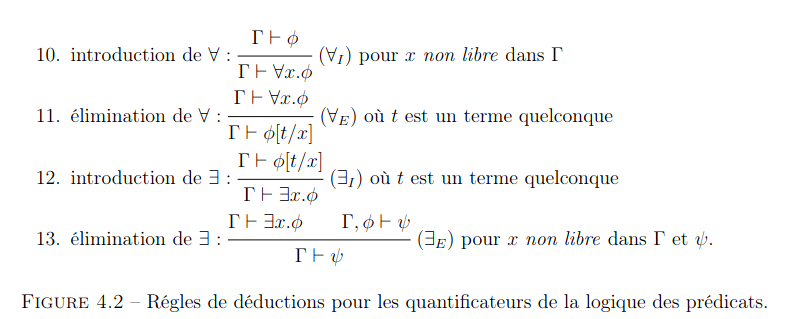
\includegraphics[scale = 0.67]{log_prop_quantificateur.png}
\end{figure}
\begin{figure}[!h]
  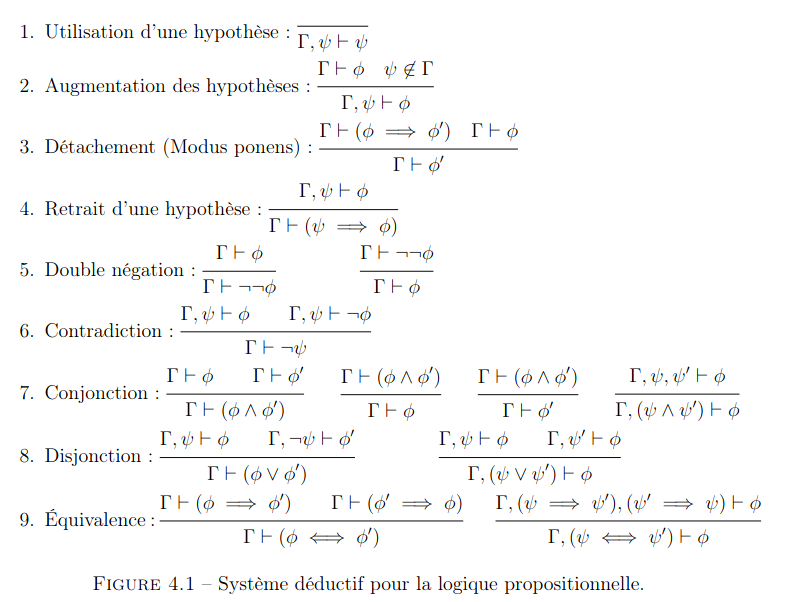
\includegraphics[scale = 0.67]{logique_propositionnelle.png}
\end{figure}
\end{document}
